

\usetikzlibrary{shadows,math}

\title{Technical Details}
\author{Fr\'ed\'eric Vogels}

\errorcontextlines 10000

\makeatletter
\pgfkeys{
  /ucll/pvm/.cd,
  start/.initial=0,
  size/.initial=1,
  height unit/.initial={0.75},
  contents/.initial={},
  id/.initial=sf,
  node style/.initial=unknown,
  stack frame/.style={minimum width=2cm,fill=red!50,font=\sc,draw},
  invisible stack frame/.style={minimum width=2cm,draw=none},
  heap object/.style={minimum width=2cm,fill=blue!50,draw},
}
\newcommand{\alloc@block}[1][]{
  {
    \pgfkeys{
      /ucll/pvm/.cd,
      #1,
      /ucll/pvm/start/.get=\ucll@start,
      /ucll/pvm/size/.get=\ucll@size,
      /ucll/pvm/height unit/.get=\ucll@heightunit,
      /ucll/pvm/contents/.get=\ucll@contents,
      /ucll/pvm/node style/.get=\ucll@nodestyle,
      /ucll/pvm/id/.get=\ucll@id,
    }
    \tikzmath{
      real \ucll@y;
      real \ucll@height;
      \ucll@y = \ucll@start * \ucll@heightunit;
      \ucll@height = \ucll@size * \ucll@heightunit;
    }
    \node[\ucll@nodestyle,minimum height={\ucll@height cm},anchor=north west,font=\tiny] (\ucll@id) at (0,-\ucll@y) {\ucll@contents};
  }
}
\newcommand{\stackframe}[1][]{
  \alloc@block[node style=/ucll/pvm/stack frame,#1]
}
\newcommand{\invisiblestackframe}[1][]{
  \alloc@block[node style=/ucll/pvm/invisible stack frame,#1,contents={}]
}
\newcommand{\heapobject}[1][]{
  \begin{scope}[xshift=2.3cm]
    \alloc@block[node style=/ucll/pvm/heap object,#1]
  \end{scope}
}

\newcommand{\memorylayout}{
  \node[anchor=south] at (1,0) {\textsc{stack}};
  \draw[fill=red!25] (-0.1,0.1) rectangle (2.1,-5.1);
  \begin{scope}[xshift=2.3cm]
    \node[anchor=south] at (1,0) {\textsc{heap}};
    \draw[fill=blue!25] (-0.1,0.1) rectangle (2.1,-5.1);
  \end{scope}
}
\makeatother

\begin{document}

\begin{frame}
  \titlepage
\end{frame}

\begin{frame}
  \frametitle{Working Example: {\tt Bar}}
  \begin{itemize}
    \item These slides contain a few step-by-step examples
    \item Make use of common struct {\tt Bar}
    \item Definition on following slide
  \end{itemize}
\end{frame}

\begin{frame}
  \frametitle{Definition of {\tt Bar}}
  \code{bar.cpp}
\end{frame}

\begin{frame}
  \frametitle{Definition of {\tt Bar}}
  \begin{itemize}
    \item Note the very unorthodox implementation
    \item Copy constructor increments fields
    \item Assignment operator triples fields
    \item \textbf{Don't do this at home!}
    \item Very ugly semantics
    \item Copy constructor should behave nicely, i.e.~just copy
    \item Same for assignment
    \item Eccentric behaviour only for illustrative purposes, to make it possible to disambiguate which member function gets called
  \end{itemize}
\end{frame}

%%% Local Variables:
%%% mode: latex
%%% TeX-master: "technical-details"
%%% End:

\begin{frame}
  \frametitle{Call By Value}
  \code[frame=lines,width=.5\linewidth,font=\small]{call-by-value.cpp}
  \begin{itemize}
    \item {\tt foo} receives a \emph{copy} of the passed object
    \item {\tt foo} knows the object's original values
    \item When {\tt foo} writes to {\tt b}, it writes to the copy
    \item {\tt foo} cannot write to the original object {\tt bar}
  \end{itemize}
\end{frame}

\begin{frame}
  \frametitle{Call By Value}
  \begin{center}
    \begin{columns}
      \column{4cm}
      \code[frame=lines,width=.95\linewidth,font=\small]{call-by-value.cpp}
      \column{4cm}
      \begin{tikzpicture}
        \memorylayout

        \only<2->{
          \stackframe[start=0,contents={bar.x = 1}]
        }
        \only<3->{
          \stackframe[start=1,contents={bar.y = 2}]
        }
        \only<5-7>{
          \stackframe[start=2,contents={b.x = 2}]
        }
        \only<8-10>{
          \stackframe[start=2,contents={b.x = 3}]
        }
        \only<6-9>{
          \stackframe[start=3,contents={b.y = 3}]
        }
      \end{tikzpicture}
    \end{columns}
  \end{center}
  \vskip2mm
  \begin{overprint}
    \onslide<1-3|handout:1-3>
    \begin{center}
      Creation of {\tt bar} on stack \\
      Default constructor is used
    \end{center}

    \onslide<4-6|handout:4-6>
    \begin{center}
      Calling {\tt foo}: {\tt bar} is passed by value \\
      $\Rightarrow$ a copy is made \\
      $\Rightarrow$ copy constructor is called
    \end{center}

    \onslide<7-8|handout:7-8>
    \begin{center}
      Incrementing {\tt b.x} operates on copy
    \end{center}

    \onslide<9-11|handout:9-11>
    \begin{center}
      Returning from {\tt foo}: all locals are cleaned up \\
      $\Rightarrow$ {\tt b}'s destructor is called \\
    \end{center}

    \onslide<12|handout:12>
    \begin{center}
      Note how {\tt bar} is still in its original state
    \end{center}
  \end{overprint}
\end{frame}


%%% Local Variables:
%%% mode: latex
%%% TeX-master: "technical-details"
%%% End:

\begin{frame}
  \frametitle{Call By Pointer}
  \code[frame=lines,width=.5\linewidth,font=\small]{call-by-pointer.cpp}
  \begin{itemize}
    \item {\tt foo} receives a \emph{pointer} to a {\tt Bar}
    \item I.e.~{\tt foo} gets the address of a {\tt Bar} object
    \item {\tt foo} can read the object by dereferencing
          \begin{itemize}
            \item {\tt *p} yields the {\tt Bar} object itself
            \item {\tt (*p).x} or {\tt p->x} are equivalent
          \end{itemize}
    \item {\tt foo} can also write to the object
          \begin{itemize}
            \item E.g.~{\tt p->x = 5}
          \end{itemize}
  \end{itemize}
\end{frame}

\begin{frame}
  \frametitle{Call By Pointer}
  \begin{center}
    \begin{columns}
      \column{4cm}
      \code[frame=lines,width=.95\linewidth,font=\small]{call-by-pointer.cpp}
      \column{4cm}
      \begin{tikzpicture}
        \memorylayout

        \only<2-6>{
          \stackframe[start=0,contents={bar.x = 1},id=bar]
        }
        \only<7->{
          \stackframe[start=0,contents={bar.x = 2},id=bar]
        }
        \only<3->{
          \stackframe[start=1,contents={bar.y = 2}]
        }
        \only<5-8>{
          \stackframe[start=2,contents={p},id=p]
          \draw[-latex] (p.east) to [bend right=30] (bar.east);
        }
      \end{tikzpicture}
    \end{columns}
  \end{center}
  \vskip2mm
  \begin{overprint}
    \onslide<1-3>
    \begin{center}
      Creation of {\tt bar} on stack \\
      Default constructor does the job
    \end{center}

    \onslide<4-5>
    \begin{center}
      Calling {\tt foo}: {\tt bar} is passed by pointer \\
      $\Rightarrow$ no copy is made \\
      $\Rightarrow$ no constructor gets called
    \end{center}

    \onslide<6-7>
    \begin{center}
      Incrementing {\tt p->x} operates on original
    \end{center}

    \onslide<8-9>
    \begin{center}
      Returning from {\tt foo}: all locals are cleaned up \\
      Only local variable is {\tt p}, a pointer \\
      A pointer's destructor does nothing
    \end{center}

    \onslide<10>
    \begin{center}
      Note how {\tt bar} has changed since before the call to {\tt foo}
    \end{center}
  \end{overprint}
\end{frame}



%%% Local Variables:
%%% mode: latex
%%% TeX-master: "technical-details"
%%% End:

\begin{frame}
  \frametitle{Call By Reference}
  \code[frame=lines,width=.5\linewidth,font=\small]{call-by-reference.cpp}
  \begin{itemize}
    \item {\tt foo} receives a \emph{reference} to a {\tt Bar}
    \item I.e.~{\tt foo} gets the address of a {\tt Bar} object
    \item {\tt foo} can read the object
          \begin{itemize}
            \item {\tt p} yields the {\tt Bar} object itself
            \item {\tt p.x} reads the {\tt x} member variable
          \end{itemize}
    \item {\tt foo} can also write to the object
          \begin{itemize}
            \item E.g.~{\tt p.x = 5}
          \end{itemize}
    \item {\tt foo} can do the same as with call-by-pointer
    \item Call-by-pointer and call-by-reference differ in syntax, but not much more
  \end{itemize}
\end{frame}

\begin{frame}
  \frametitle{Call By Reference}
  \begin{center}
    \begin{columns}
      \column{4cm}
      \code[frame=lines,width=.95\linewidth,font=\small]{call-by-reference.cpp}
      \column{4cm}
      \begin{tikzpicture}
        \memorylayout

        \only<2-6>{
          \stackframe[start=0,contents={bar.x = 1},id=bar]
        }
        \only<7->{
          \stackframe[start=0,contents={bar.x = 2},id=bar]
        }
        \only<3->{
          \stackframe[start=1,contents={bar.y = 2}]
        }
        \only<5-8>{
          \stackframe[start=2,contents={b},id=p]
          \draw[-latex] (p.east) to [bend right=30] (bar.east);
        }
      \end{tikzpicture}
    \end{columns}
  \end{center}
  \vskip2mm
  \begin{overprint}
    \onslide<1-3>
    \begin{center}
      Creation of {\tt bar} on stack \\
      Default constructor does the job
    \end{center}

    \onslide<4-5>
    \begin{center}
      Calling {\tt foo}: {\tt bar} is passed by reference \\
      $\Rightarrow$ no copy is made \\
      $\Rightarrow$ no constructor gets called
    \end{center}

    \onslide<6-7>
    \begin{center}
      Incrementing {\tt b.x} operates on original
    \end{center}

    \onslide<8-9>
    \begin{center}
      Returning from {\tt foo}: all locals are cleaned up \\
      Only local variable is {\tt b}, a reference \\
      A reference's destructor does nothing
    \end{center}

    \onslide<10>
    \begin{center}
      Note how {\tt bar} has changed since before the call to {\tt foo}
    \end{center}
  \end{overprint}
\end{frame}



%%% Local Variables:
%%% mode: latex
%%% TeX-master: "technical-details"
%%% End:

\begin{frame}
  \frametitle{Return By Value}
  \code[frame=lines,width=.5\linewidth,font=\small]{return-by-value.cpp}
  \begin{itemize}
    \item {\tt foo} returns a {\tt Bar}
    \item This means it returns it \emph{by value}
    \item A copy must be made
    \item This copy is made using a copy constructor
    \item In reality, things are more complex
          \begin{itemize}
            \item Compiler can optimise: have {\tt foo} directly write to {\tt bar}
            \item Move constructors can be used under certain circumstances
          \end{itemize}
  \end{itemize}
\end{frame}

\begin{frame}
  \frametitle{Return By Value}
  \begin{center}
    \begin{columns}
      \column{4cm}
      \code[frame=lines,width=.95\linewidth,font=\small]{return-by-value.cpp}
      \column{4cm}
      \begin{tikzpicture}
        \memorylayout

        \only<2->{
          \stackframe[start=0,contents={bar.x = ?}]
        }
        \only<3->{
          \stackframe[start=1,contents={bar.y = ?}]
        }
        \only<6->{
          \stackframe[start=2,contents={b.x = 1}]
        }
        \only<7->{
          \stackframe[start=3,contents={b.y = 2}]
        }
      \end{tikzpicture}
    \end{columns}
  \end{center}
  \vskip2mm
  \begin{overprint}
    \onslide<1-3|handout:1-3>
    \begin{center}
      Space for {\tt bar} is allocated on stack \\
      {\tt bar} is \emph{not} initialised yet \\
      We have to wait for {\tt foo()}'s result
    \end{center}

    \onslide<4|handout:4>
    \begin{center}
      {\tt foo} gets called.
    \end{center}

    \onslide<5-7|handout:5-7>
    \begin{center}
      {\tt b} gets created on the stack.
    \end{center}

    \onslide<8|handout:8>
    \begin{center}
      What happens next depends on your compiler and its optimisation settings\dots
    \end{center}
  \end{overprint}
\end{frame}

\begin{frame}
  \begin{center} \Huge
    Possible Path A \\[4mm]
    The Path of Least Optimisation
  \end{center}
\end{frame}

\begin{frame}
  \frametitle{Return By Value (Path A)}
  \begin{center}
    \begin{columns}
      \column{4cm}
      \code[frame=lines,width=.95\linewidth,font=\small]{return-by-value.cpp}
      \column{4cm}
      \begin{tikzpicture}
        \memorylayout

        \only<1-6>{
          \stackframe[start=0,contents={bar.x = ?}]
        }
        \only<7->{
          \stackframe[start=0,contents={bar.x = 3}]
        }
        \only<1-7>{
          \stackframe[start=1,contents={bar.y = ?}]
        }
        \only<8-13>{
          \stackframe[start=1,contents={bar.y = 4}]
        }
        \only<1-12>{
          \stackframe[start=2,contents={b.x = 1}]
        }
        \only<1-11>{
          \stackframe[start=3,contents={b.y = 2}]
        }
        \only<2-10>{
          \stackframe[start=4,contents={temp.x = 2}]
        }
        \only<3-9>{
          \stackframe[start=5,contents={temp.y = 3}]
        }
      \end{tikzpicture}
    \end{columns}
  \end{center}
  \vskip2mm
  \begin{overprint}
    \onslide<1-3|handout:1-3>
    \begin{center}
      Returning {\tt b} creates a copy of {\tt b} \\
      Let's call it {\tt temp} \\
    \end{center}

    \onslide<4|handout:4>
    \begin{center}
      {\tt temp} is considered the object that is returned by {\tt foo}
    \end{center}

    \onslide<5|handout:5>
    \begin{center}
      We can continue initialising {\tt bar}. \\
      If declaration and assignment occur on the same line (as is the case here),
      the copy constructor is called.
    \end{center}

    \onslide<6-8|handout:6-8>
    \begin{center}
      The copy constructor is called with a reference to {\tt temp} as its argument
    \end{center}

    \onslide<9-13|handout:9-13>
    \begin{center}
      {\tt temp} and {\tt b} are cleaned up \\
      {\tt \~{}Bar()} is called twice
    \end{center}
  \end{overprint}
\end{frame}

\begin{frame}
  \begin{center} \Huge
    Possible Path B \\[4mm]
    Return Value Optimisation (RVO)
  \end{center}
\end{frame}

\begin{frame}
  \frametitle{Return By Value (Path B)}
  \begin{center}
    \begin{columns}
      \column{4cm}
      \code[frame=lines,width=.95\linewidth,font=\small]{return-by-value.cpp}
      \column{4cm}
      \begin{tikzpicture}
        \memorylayout

        \only<1-2>{
          \stackframe[start=0,contents={bar.x = ?}]
        }
        \only<3->{
          \stackframe[start=0,contents={bar.x = 2}]
        }
        \only<1-3>{
          \stackframe[start=1,contents={bar.y = ?}]
        }
        \only<4->{
          \stackframe[start=1,contents={bar.y = 3}]
        }
        \only<1-6>{
          \stackframe[start=2,contents={b.x = 1}]
        }
        \only<1-5>{
          \stackframe[start=3,contents={b.y = 2}]
        }
      \end{tikzpicture}
    \end{columns}
  \end{center}
  \vskip2mm
  \begin{overprint}
    \onslide<1|handout:1>
    \begin{center}
      The compiler is allowed to omit making a copy of {\tt b} prior to returning it \\
      {\tt b} is then considered the object that is returned
    \end{center}

    \onslide<2-4|handout:2-4>
    \begin{center}
      The copy constructor initialising {\tt bar} is called with a reference to {\tt b} as argument
    \end{center}

    \onslide<5-7|handout:5-7>
    \begin{center}
      {\tt b}'s destructor is called
    \end{center}
  \end{overprint}
\end{frame}

\begin{frame}
  \begin{center} \Huge
    Possible Path C \\[4mm]
    Full Optimisation
  \end{center}
\end{frame}

\begin{frame}
  \frametitle{Return By Value (Path C)}
  \begin{center}
    \begin{columns}
      \column{4cm}
      \code[frame=lines,width=.95\linewidth,font=\small]{return-by-value.cpp}
      \column{4cm}
      \begin{tikzpicture}
        \memorylayout

        \only<1-3>{
          \stackframe[start=0,contents={bar.x = ?},id=bar]
        }
        \only<4->{
          \stackframe[start=0,contents={bar.x = 1},id=bar]
        }
        \only<1-4>{
          \stackframe[start=1,contents={bar.y = ?}]
        }
        \only<5->{
          \stackframe[start=1,contents={bar.y = 2}]
        }
        \only<1-6>{
          \stackframe[start=2,contents={b},id=b]
          \draw[-latex] (b.east) to [bend right=30] (bar.east);
        }
      \end{tikzpicture}
    \end{columns}
  \end{center}
  \vskip2mm
  \begin{overprint}
    \onslide<1|handout:1>
    \begin{center}
      It is not necessary for {\tt foo} to have its own object {\tt b}.
      Instead, it can operate directly on {\tt bar}.
    \end{center}

    \onslide<2|handout:2>
    \begin{center}
      Every write that {\tt foo} makes to {\tt b}
      is then in reality a write to {\tt bar}
    \end{center}

    \onslide<3-5|handout:3-5>
    \begin{center}
      When {\tt foo} initialised {\tt b} using the default constructor,
      it is in reality initialising {\tt bar}
    \end{center}

    \onslide<6-7|handout:6-7>
    \begin{center}
      When {\tt foo} ends, {\tt b} is cleaned up.
      Since {\tt b} was never constructed as a separate object, {\tt b} cannot be destructed either.
      In other words, {\tt b} just disappears. {\tt b} can be seen as a reference to {\tt bar}.
    \end{center}
  \end{overprint}
\end{frame}

\begin{frame}
  \begin{center} \Huge
    Possible Path D \\[4mm]
    Move Constructor
  \end{center}
\end{frame}

\begin{frame}
  \frametitle{Return By Value (Path D)}
  \begin{itemize}
    \item If a move constructor is defined, {\tt b}
          may be \emph{moved} to {\tt bar}
    \item Steps:
          \begin{enumerate}
            \item {\tt b} gets created with the default constructor
            \item Upon returning, {\tt bar} gets initialised with its move constructor.
                  It ``steals'' {\tt b}'s data
            \item {\tt b} is destructed
          \end{enumerate}
    \item We don't discuss move constructors in detail for this course
  \end{itemize}
\end{frame}

\begin{frame}
  \frametitle{Return By Value: Summary}
  \begin{itemize}
    \item It is impossible to predict what exactly will happen
    \item Four possibilities
          \begin{itemize}
            \item Two copy constructors called
            \item One copy constructor called
            \item Zero constructors called
            \item One move constructors called
          \end{itemize}
    \item It is therefore important to define your constructors in such a way
          that it does not matter how often they get called
    \item A copy constructor should only copy and do nothing more
    \item Then it does not matter if you get an object, a copy of an object, or a copy of a copy of an object
    \item {\tt Bar}'s implementation clearly does not satisfy this requirement
  \end{itemize}
\end{frame}

%%% Local Variables:
%%% mode: latex
%%% TeX-master: "technical-details"
%%% End:

\begin{frame}
  \frametitle{Returning a Local Variable By Pointer}
  \code[frame=lines,width=.5\linewidth,font=\small]{return-local-by-pointer.cpp}
  \begin{itemize}
    \item Returning by pointer is possible (why would it not be?)
    \item Returning a \emph{local} by pointer is an extremely bad idea (leads to undefined behaviour)
    \item The local gets removed after the function has returned\dots
    \item \dots yet the pointer  will still point to that space
    \item A pointer pointing to something that's been destroyed is called a dangling pointer
  \end{itemize}
\end{frame}

\begin{frame}
  \frametitle{Return Local By Pointer}
  \begin{center}
    \begin{columns}
      \column{4cm}
      \code[frame=lines,width=.95\linewidth,font=\small]{return-local-by-pointer.cpp}
      \column{4cm}
      \begin{tikzpicture}
        \memorylayout

        \only<2-7>{
          \stackframe[start=0,contents={p = ?}]
        }
        \only<5-10>{
          \stackframe[start=1,contents={b.x = 1},id=b]
        }
        \only<11->{
          \invisiblestackframe[start=1,contents={b.x = 1},id=b]
        }
        \only<6-9>{
          \stackframe[start=2,contents={b.y = 2}]
        }        
        \only<8->{
          \stackframe[start=0,contents={p},id=p]
          \draw[-latex] (p.east) to [bend left=30] (b.east);
        }
      \end{tikzpicture}
    \end{columns}
  \end{center}
  \vskip2mm
  \begin{overprint}
    \onslide<1-2>
    \begin{center}
      Space gets allocated (but not initialised, that's for later) for {\tt p}
    \end{center}

    \onslide<3>
    \begin{center}
      {\tt foo} gets called.
    \end{center}

    \onslide<4-6>
    \begin{center}
      {\tt b} gets created on the stack.
    \end{center}

    \onslide<7-8>
    \begin{center}
      {\tt foo} returns the address of {\tt b}
    \end{center}

    \onslide<9-11>
    \begin{center}
      {\tt foo}'s locals get cleaned up \\
      {\tt b}'s destructor gets called
    \end{center}

    \onslide<12>
    \begin{center}
      {\tt p} points to no-man's-land \\
      {\tt p->x++} is undefined
    \end{center}
  \end{overprint}
\end{frame}

\begin{frame}
  \frametitle{Returning Local by Reference}
  \begin{itemize}
    \item Returning a local by reference suffers from exactly the same problem
  \end{itemize}
\end{frame}


%%% Local Variables:
%%% mode: latex
%%% TeX-master: "technical-details"
%%% End:

\begin{frame}
  \frametitle{Returning by Pointer or Reference}
  \begin{itemize}
    \item When is it ok to return a pointer or reference?
    \item Whenever the object pointed to still exists after the function cleans up
    \item E.g.~it can return a pointer/reference to a heap-allocated object
    \item It can return a pointer/reference to an object
          it received by pointer/reference (see examples on next slides)
  \end{itemize}
\end{frame}

\begin{frame}
  \frametitle{Returning Heap-Allocated Object By Pointer}
  \begin{center}
    \begin{columns}
      \column{5cm}
      \code[frame=lines,width=.95\linewidth,font=\small]{return-heap-by-pointer.cpp}
      \column{4cm}
      \begin{tikzpicture}
        \memorylayout

        \only<2-10>{
          \stackframe[start=0,contents={p = ?}]
        }
        \only<5-8>{
          \stackframe[start=1,contents={q = ?}]
        }
        \only<7->{
          \heapobject[start=0,contents={Bar(x=1,y=2)},id=bar];
        }
        \only<9-12>{
          \stackframe[start=1,contents={q},id=q]
          \draw[-latex] (q.east) -- (bar.west);
        }
        \only<11->{
          \stackframe[start=0,contents={p},id=p]
          \draw[-latex] (p.east) -- (bar.west);
        }
      \end{tikzpicture}
    \end{columns}
  \end{center}
  \vskip2mm
  \begin{overprint}
    \onslide<1-2|handout:1-2>
    \begin{center}
      Space gets allocated (but not initialised) for {\tt p}
    \end{center}

    \onslide<3|handout:3>
    \begin{center}
      {\tt foo} gets called.
    \end{center}

    \onslide<4-5|handout:4-5>
    \begin{center}
      {\tt q} gets allocated on the stack
    \end{center}

    \onslide<6-7|handout:6-7>
    \begin{center}
      {\tt b} gets created on the heap.
    \end{center}

    \onslide<8-9|handout:8-9>
    \begin{center}
      {\tt q} points to the newly created heap-object
    \end{center}

    \onslide<10-11|handout:10-11>
    \begin{center}
      {\tt foo} returns {\tt q} \\
      The address it contains gets copied to {\tt p}
    \end{center}

    \onslide<12-13|handout:12-13>
    \begin{center}
      {\tt foo}'s locals get cleaned up \\
      {\tt q} is the only local, and since it is a {\tt Bar*}, nothing happens (i.e.~no destructors)
    \end{center}
  \end{overprint}
\end{frame}

\begin{frame}
  \frametitle{Returning Heap Objects by Reference}
  \code{return-heap-by-reference.cpp}
  \begin{itemize}
    \item This works, but it's rather unidiomatic
    \item It makes more sense to return a pointer
    \item Or better yet, a {\tt std::shared\_ptr}
  \end{itemize}
\end{frame}


%%% Local Variables:
%%% mode: latex
%%% TeX-master: "technical-details"
%%% End:

\begin{frame}
  \frametitle{Returning An Argument By Reference}
  \code[width=.5\linewidth]{return-arg-by-reference.cpp}
  \begin{itemize}
    \item If a function receives an object by ptr/ref, it means
          this object will survive the function
    \item Hence, the function can return a ptr/ref to this object
    \item It's a bit strange to do, but it can come in handy
  \end{itemize}
\end{frame}

\begin{frame}
  \frametitle{Returning An Argument By Reference}
  \begin{center}
    \begin{columns}
      \column{5cm}
      \code[frame=lines,width=.95\linewidth,font=\small]{return-arg-by-reference.cpp}
      \column{4cm}
      \begin{tikzpicture}
        \memorylayout

        \only<2->{
          \stackframe[start=0,contents={bar.x = 1},id=bar]
        }
        \only<3->{
          \stackframe[start=1,contents={bar.y = 2}]
        }
        \only<5-8>{
          \stackframe[start=2,contents={p = ?}]
        }
        \only<9->{
          \stackframe[start=2,contents={p},id=p]
          \draw[-latex] (p.east) to [bend right=30] (bar.east);
        }
        \only<7-10>{
          \stackframe[start=3,contents={b},id=b]
          \draw[-latex] (b.east) to [bend right=30] (bar.east);
        }
      \end{tikzpicture}
    \end{columns}
  \end{center}
  \vskip2mm
  \begin{overprint}
    \onslide<1-3|handout:1-3>
    \begin{center}
      {\tt bar} gets created on stack (default constructor)
    \end{center}

    \onslide<4-5|handout:4-5>
    \begin{center}
      {\tt p} gets allocated on the stack (uninitialised)
    \end{center}

    \onslide<6-7|handout:6-7>
    \begin{center}
      {\tt foo} gets called, argument {\tt b} resides on heap
    \end{center}

    \onslide<8-9|handout:8-9>
    \begin{center}
      {\tt foo} returns address of what {\tt b} refers to, which is {\tt bar} \\
      {\tt p} is overwritten with this address
    \end{center}

    \onslide<10-11|handout:10-11>
    \begin{center}
      {\tt foo} is done, cleanup time
    \end{center}

  \end{overprint}
\end{frame}



%%% Local Variables:
%%% mode: latex
%%% TeX-master: "technical-details"
%%% End:

\begin{frame}
  \frametitle{Assignment Operator}
  \code[width=.5\linewidth]{assignment.cpp}
  \begin{itemize}
    \item {\tt x = y} where {\tt x} and {\tt y} are objects (not pointers/references)
          copies the contents of {\tt y} to {\tt x}
    \item The {\tt =} operator will generally overwrite all of {\tt x}'s fields with {\tt y}'s field values.
    \item It is important to distinguish between using {\tt =} on objects and using {\tt =} on pointers
  \end{itemize}
\end{frame}

\begin{frame}
  \frametitle{Assignment Operator On Objects}
  \begin{center}
    \begin{columns}
      \column{5cm}
      \code[frame=lines,width=.95\linewidth,font=\small]{assignment.cpp}
      \column{4cm}
      \begin{tikzpicture}
        \memorylayout
        
        \only<2-7>{
          \stackframe[start=0,contents={bar.x = 1}]
        }
        \only<8->{
          \stackframe[start=0,contents={bar.x = 3}]
        }
        \only<3-8>{
          \stackframe[start=1,contents={bar.y = 2}]
        }
        \only<9->{
          \stackframe[start=1,contents={bar.y = 6}]
        }
        \only<5-11>{
          \stackframe[start=2,contents={temp.x = 1}]
        }
        \only<6-10>{
          \stackframe[start=3,contents={temp.y = 2}]
        }
      \end{tikzpicture}
    \end{columns}
  \end{center}
  \vskip2mm
  \begin{overprint}
    \onslide<1-3>
    \begin{center}
      {\tt bar} gets created on stack using the default constructor
    \end{center}

    \onslide<4-6>
    \begin{center}
      {\tt foo} gets called. It creates a new object (default constructor) which we'll call {\tt temp}.
    \end{center}

    \onslide<7-9>
    \begin{center}
      {\tt Bar::operator =} gets called on {\tt bar} with as argument a reference to {\tt temp}
    \end{center}

    \onslide<10-12>
    \begin{center}
      {\tt temp} gets destroyed (destructor gets called)
    \end{center}
  \end{overprint}
\end{frame}

%%% Local Variables:
%%% mode: latex
%%% TeX-master: "technical-details"
%%% End:

\begin{frame}
  \frametitle{Different Meanings of Assignment}
  \begin{itemize}
    \item The {\tt =} operator's meaning depends on how you use it
    \item We distinguish four cases
          \begin{itemize}
            \item Assignment at declaration
            \item Assignment between objects
            \item Assignment between pointers
            \item Assignment with references
          \end{itemize}
  \end{itemize}
\end{frame}

\begin{frame}
  \frametitle{Assignment At Declaration}
  \code[font=\small,width=.95\linewidth]{assignment-declaration.cpp}
  \begin{itemize}
    \item If assignment happens in the same statement as declaration,
          the copy constructor will be called.
  \end{itemize}
\end{frame}

\begin{frame}
  \frametitle{Assignment with Objects}
  \code[font=\small,width=.95\linewidth]{assignment-objects.cpp}
  \begin{itemize}
    \item Using {\tt x = y} where {\tt x} and {\tt y} are of type {\tt T}
          will call {\tt T::operator =(const T\&)}
    \item No new objects get constructed
  \end{itemize}
\end{frame}

\begin{frame}
  \frametitle{Assignment with Pointers}
  \code[font=\small,width=.95\linewidth]{assignment-pointers.cpp}
  \begin{itemize}
    \item Using {\tt x = y} where {\tt x} and {\tt y} are of type {\tt T*}
          will simply copy pointers
    \item This is C++'s closest equivalent of Java's assignment
    \item {\tt q} and {\tt r} point to the same object
    \item Writing {\tt p = r} would make {\tt p} also point to the same object as {\tt q} and {\tt r}.
          {\tt bar} would remain untouched.
    \item Neither copy constructor nor {\tt Bar::operator =} is called
  \end{itemize}
\end{frame}

\begin{frame}
  \frametitle{Assignment with References}
  \code[font=\small,width=.95\linewidth]{assignment-references.cpp}
  \begin{itemize}
    \item When declaring a reference, immediate initialisation is mandatory (see {\tt bar5})
    \item Declaring reference is same as introducing extra name for same object
    \item {\tt bar} and {\tt bar2} are indistuingishable from each other
    \item When working with a reference, it is the same as if working with the original object
    \item {\tt bar2 = bar3} is the same as {\tt bar = bar3}: calls {\tt operator=}
    \item You cannot make a reference refer to another object. Once it refers to some object,
          it will do so until it dies.
  \end{itemize}
\end{frame}



%%% Local Variables:
%%% mode: latex
%%% TeX-master: "technical-details"
%%% End:


\end{document}


%%% Local Variables:
%%% mode: latex
%%% TeX-master: "technical-details"
%%% End:
